% Chapter 2

\chapter{Methodology} % Write in your own chapter title
\label{Chapter3}
\lhead{Chapter 3. \emph{Approach of Weather Classification}}

\section{Dataset}

There are over 15 million labeled images in ImageNet database belonging to about 22,000 categories. The images were collected from the Internet and labeled manually. From 2010, an annual competition named the ImageNet Large-Scale Visual REcognition Challenge (ILSVRC) has been held. The competition uses a subset of dataset which is 1000 images in 1000 categories. Totally, there are over 1 million training images and 50,000 validation images and 150,000 images for testing.
\graphicspath{ {./Figures/} }
\begin{figure}[!htb]
    \centering
	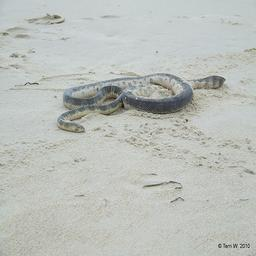
\includegraphics[width=0.4\textwidth]{ILSVRC2012_val_00000001.JPEG}
    \qquad
    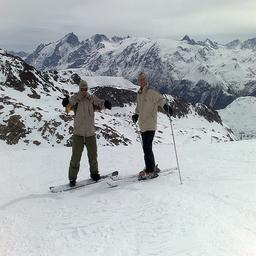
\includegraphics[width=0.4\textwidth]{ILSVRC2012_val_00000002.JPEG}
    \caption{2 Figures from ImageNet}%
    \label{fig:ImageNetExamples}%
\end{figure}

For weather dataset, it contains 10,000 images for two categories evenly, cloudy and sunny. They are from three sources, Sun Dataset\citep{russell2008labelme}, Labelme Dataset\citep{xiao2010sun} and Flickr. They were classified manually and similar images are removed. There are no unambiguous images.
\graphicspath{ {./Figures/} }
\begin{figure}[!htb]
    \centering
	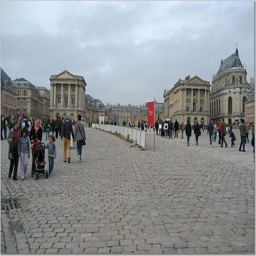
\includegraphics[width=0.4\textwidth]{cloudy_0001.png}
    \qquad
    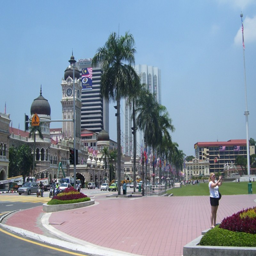
\includegraphics[width=0.4\textwidth]{sunny_0003.png}
    \caption{2 Figures from Weather Dataset}%
    \label{fig:WeatherExamples}%
\end{figure}

The two datasets are different. ImageNet dataset is for object classification and weather dataset is for scenes classification. Because the two datasets consists of different resolution images, we have to resize them to a fixed resolution of $256x256$ for constant dimension input for neural networks. To train the model with ImageNet images, we resize shorter side of images to length 256 and then cropped out a $256x256$ image from center.


\section{Convolutional Neural Networks Architecture}

Due to the significant performance of AlexNet \citep{krizhevsky2012imagenet} deep convolutional neural networks, we train a model based on it. The architecture of the network has seven hidden adaptive layers-five convolutional and two fully connected layers.
\begin{figure}[!htb]
    \centering
	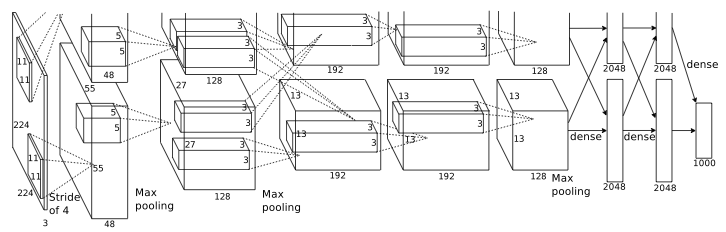
\includegraphics[width=0.8\textwidth]{AlexNet.png}
    \caption{Architecture of AlexNet}%
    \label{fig:ImageNetArch}%
\end{figure}
The network is very deep and the early layers are split over on two GPUs. It is able to give $62.5\%$ accuracy rates with one prediction and $83\%$ accuracy rates with five predictions.

The network replaces each neuron's outputs nonlinearity function $f$ from $f(x) = tanh(x)$ or $f(x) = (1 + e^{-x})^(-1)$ to Rectified Linear Units(RELUs)\citep{nair2010rectified} which can accelerate learning speed several times faster than $tanh$ function. 

In the network, there are three types of layers and they play different roles in the model. The input data dimension is $224x224x3$ which means the raw pixel value stored in a width 224, height 224 and with three color channels R,G,B matrix. In the first convolutional layer, there are 98 kernel of size $11x11$ with stride size 4 and outputs are 96 neurons. A max pooling layer with kernel $3x3$ and stride size 2 downsamples the spatial dimensions to $112x112x96$. The second convolutional layer filters output of previous pooling layer with kernel size $5x5$ with stride size 1.


















